%chargedCorrBtoLambdaPlots
%!TEX root = ../main.tex
%

\subsection{$B^- \rightarrow \bar{\Lambda_c}^-$ decays: additional plots}
%\section{$B^- \rightarrow \Lambda_c^+$ decays: additional plots}%\label{}
\label{sec:chargedAnticorrApp}

\begin{figure}[H]
  \begin{subfigure}{14.5cm}
    \centering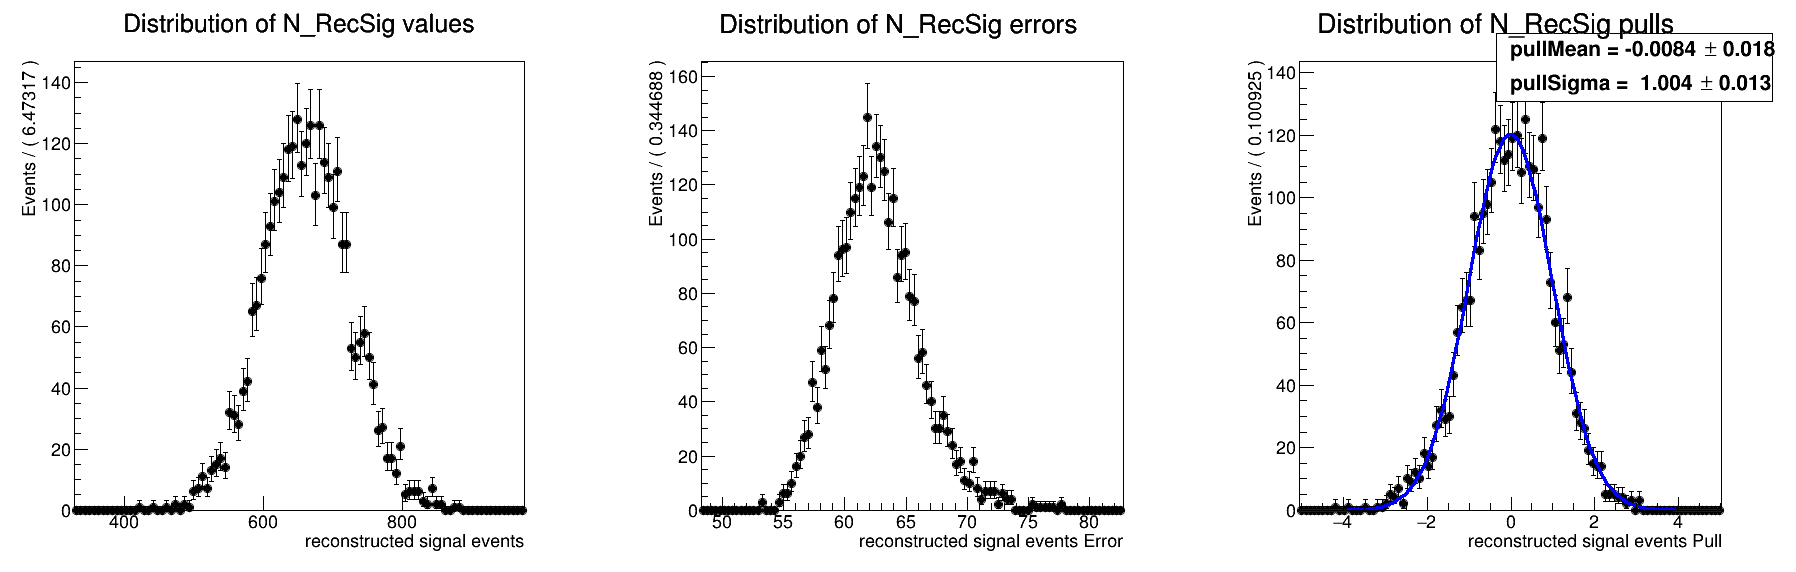
\includegraphics[width=13.8cm]{A3-Appendix/figs/2DanticorrLambdaC_NrecSig_mcstudy.png}
   % \caption{Fit on $M(p K \pi)$ in the region $5.25 < M_{bc} < 5.258$ GeV/c$^2$.  }
   % \label{fig:CrossfeedMbcRegionsInvMpeak1}
  \end{subfigure}
  \begin{subfigure}{14.5cm}
    \centering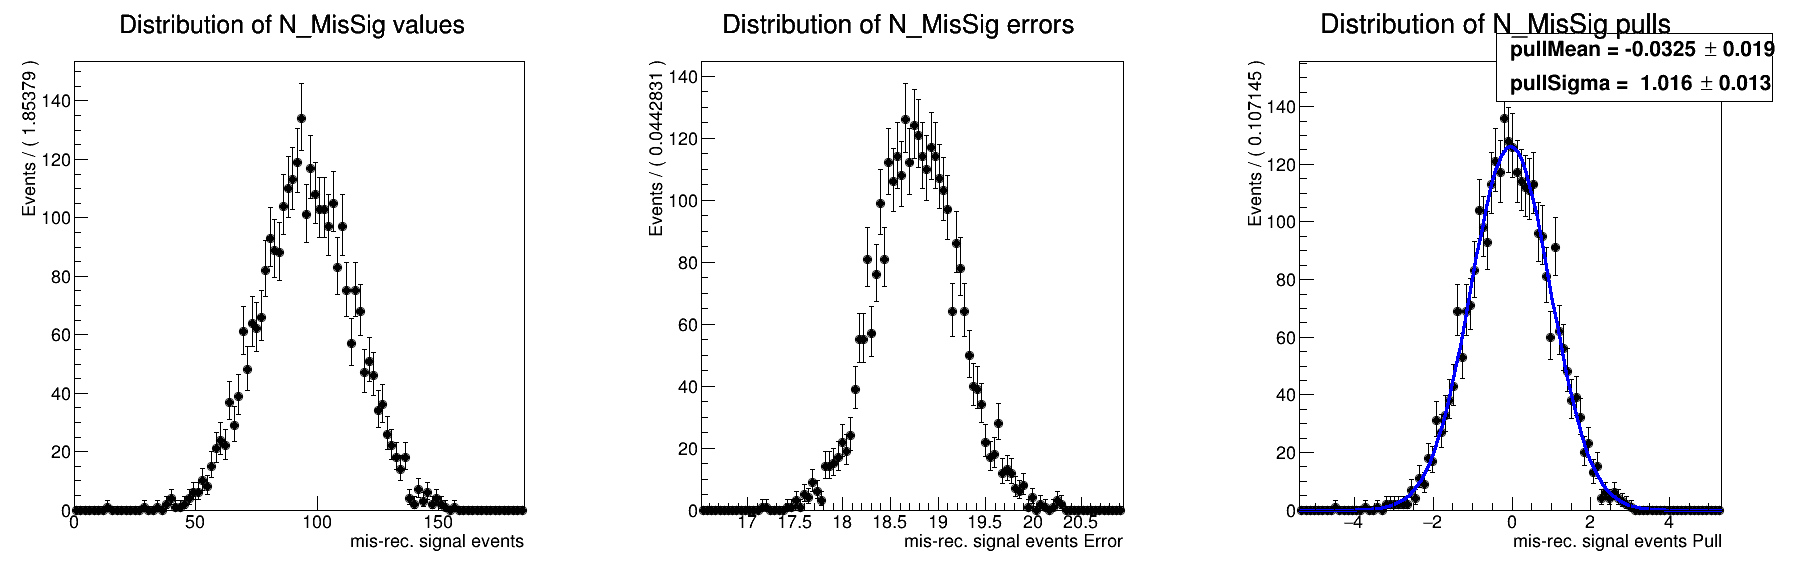
\includegraphics[width=13.8cm]{A3-Appendix/figs/2DanticorrLambdaC_NmisSig_mcstudy.png}
  \end{subfigure}
 
  \begin{subfigure}{14.5cm}
    \centering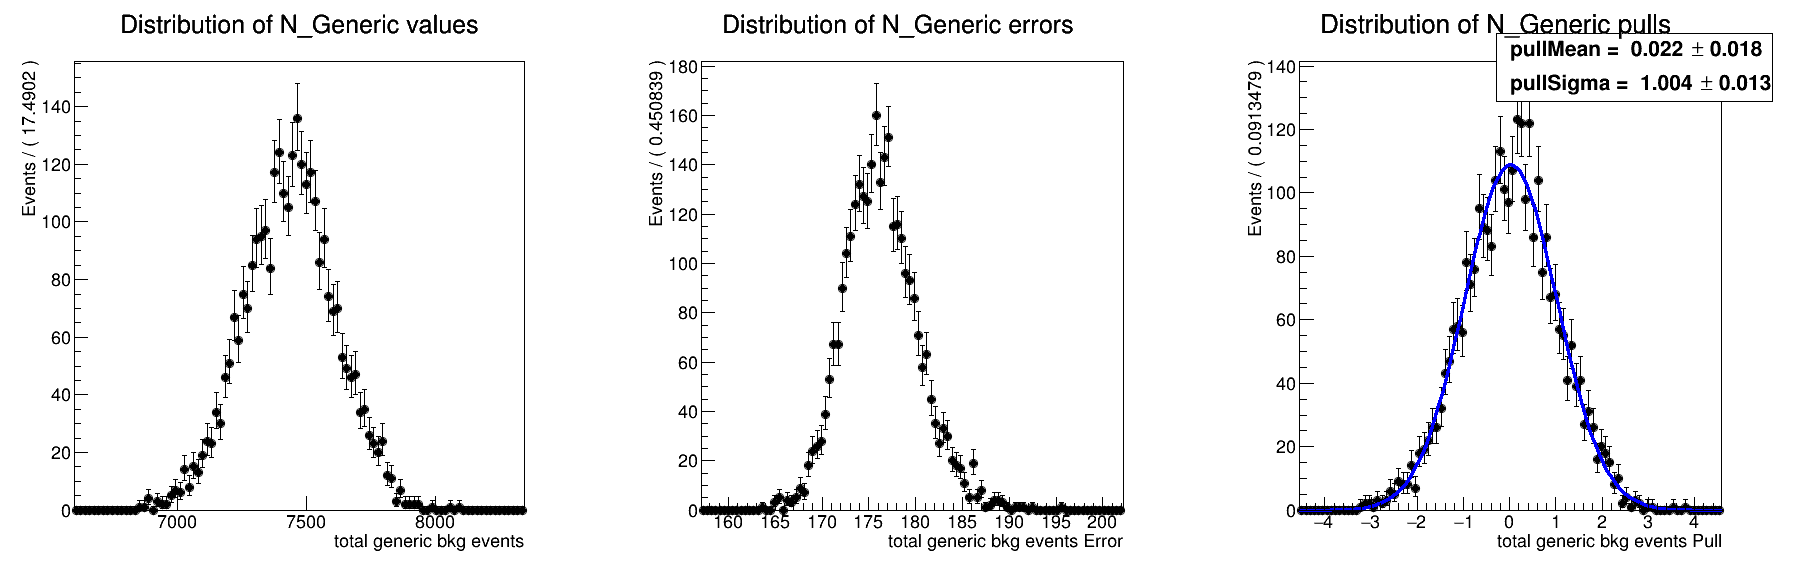
\includegraphics[width=13.8cm]{A3-Appendix/figs/2DanticorrLambdaC_N_Generic_mcstudy.png}
  \end{subfigure}
  \begin{subfigure}{14.5cm}
    \centering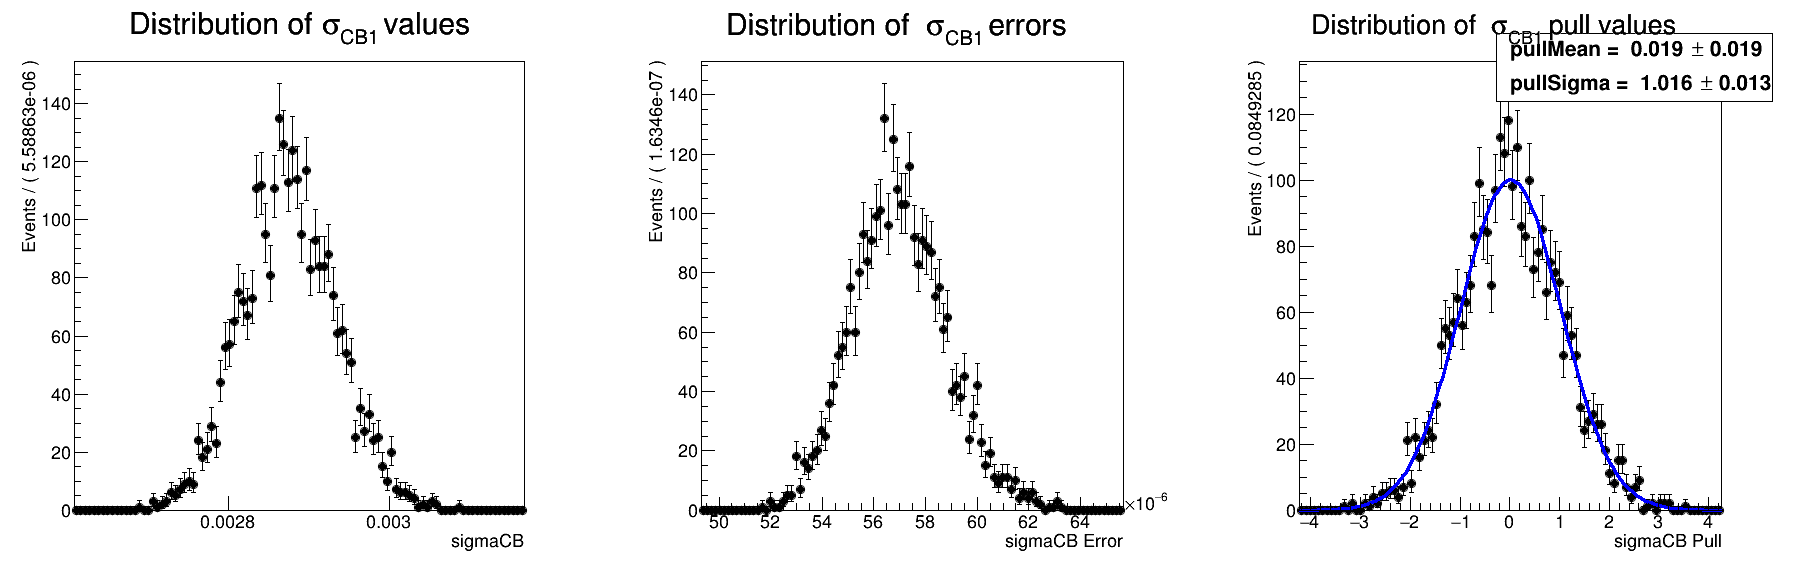
\includegraphics[width=13.8cm]{A3-Appendix/figs/2DanticorrLambdaC_sigmaCB1_mcstudy.png}
  \end{subfigure}
  \begin{subfigure}{14.5cm}
    \centering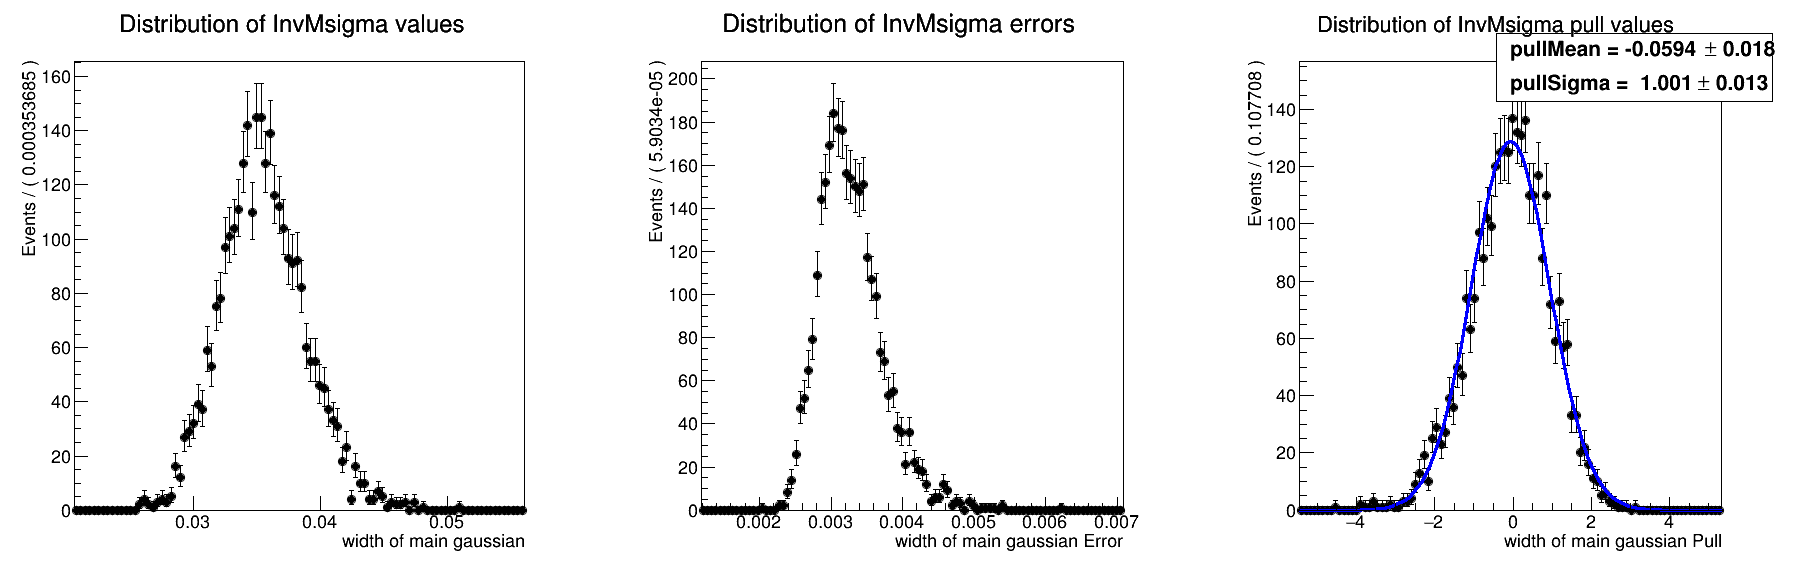
\includegraphics[width=13.8cm]{A3-Appendix/figs/2DanticorrLambdaC_InvMsigma_mcstudy.png}
    %\label{fig:CrossfeedMbcRegionsInvMpeak5}
  \end{subfigure}
  %\label{fig:CrossfeedMbcRegionsInvMpeak}
  \caption{Toy MC study for the two dimensional fit model described in Sec.  \ref{sec:chargedAnticorr2DtotalFit}}
\end{figure}



\begin{figure}[h!]
%\centering
{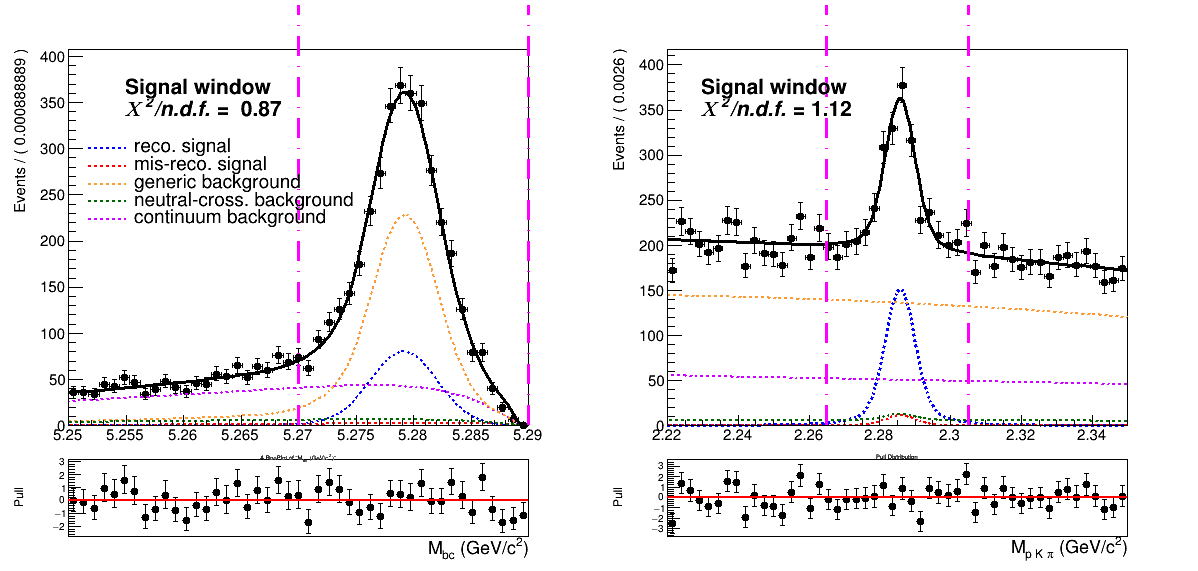
\includegraphics[width=0.75\textwidth]{A3-Appendix/figs/Signal_window_Total_2DFit_stream0_chargedAnticorrLambdaC_Crossfeed_fraction.png}}
\caption{Signal region ($2.22 < M(p K \pi) < 2.35$ GeV/c$^2$ and $5.27 < M_{bc} < 5.29$ GeV/c$^2$ ) projections of the dimensional fit on stream 0 Monte Carlo simulated data.}
\label{fig:stream0_sig_window_Total2Dfit_charged_anticorrLambdaC}
\end{figure}

\begin{figure}[h!]
%\centering
{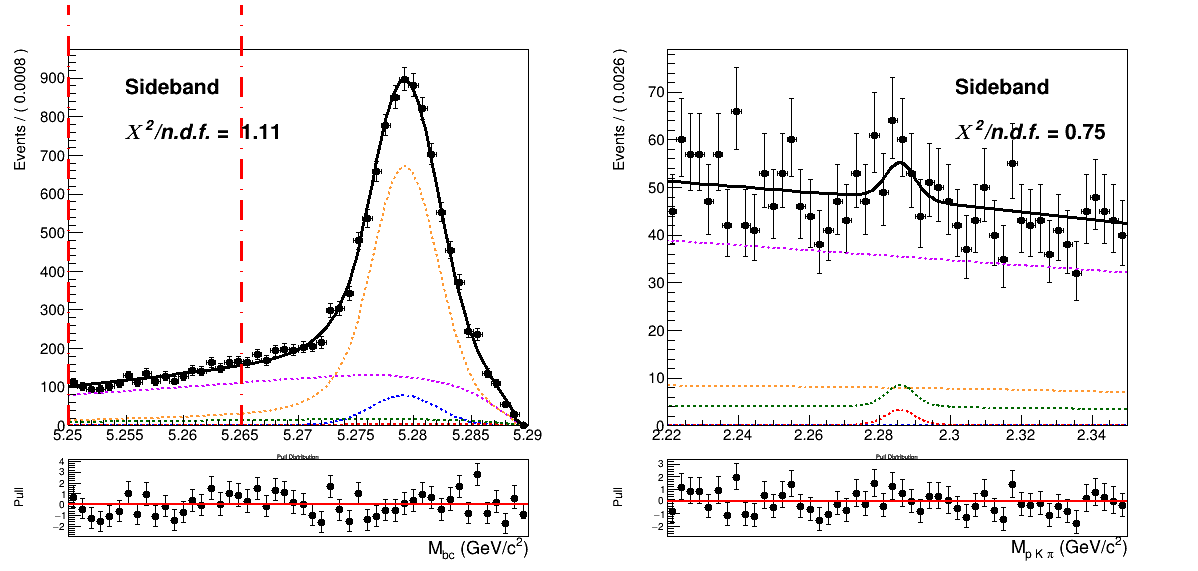
\includegraphics[width=0.75\textwidth]{A3-Appendix/figs/Mbc_Sideband_Total_2DFit_stream0_chargedAnticorrLambdaC_Crossfeed_fraction.png}}
\caption{Sideband region of $5.25 < M_{bc} < 5.265$ GeV/c$^2$ projection of the two dimensional fit on stream 0 Monte Carlo simulated data.}
\label{fig:stream0_MbcSideband_Total2Dfit_charged_anticorrLambdaC}
\end{figure}

\begin{figure}[b]
%\centering
{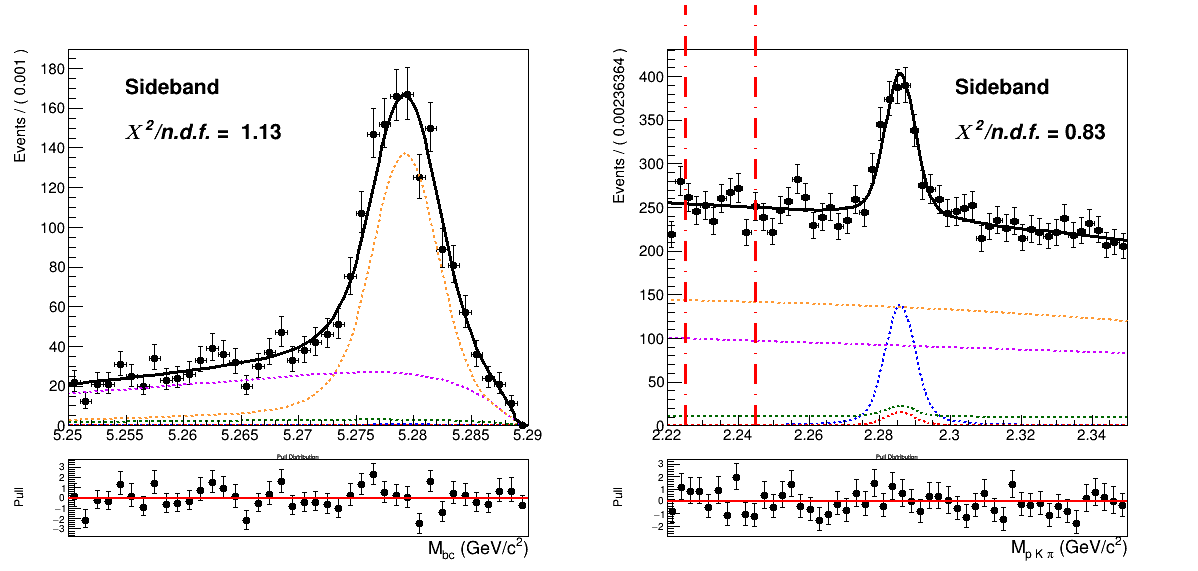
\includegraphics[width=0.75\textwidth]{A3-Appendix/figs/InvM_Sideband2_Total_2DFit_stream0_chargedAnticorrLambdaC_Crossfeed_fraction.png}}
\caption{Sideband region of $2.22 < M(p K \pi) < 2.35$ GeV/c$^2$ projection of the two dimensional fit on stream 0 Monte Carlo simulated data.}
\label{fig:stream0_InvMSideband_Total2Dfit_charged_anticorrLambdaC}
\end{figure}

\newpage

\begin{figure}[h!]
  \begin{subfigure}{15cm}
    \centering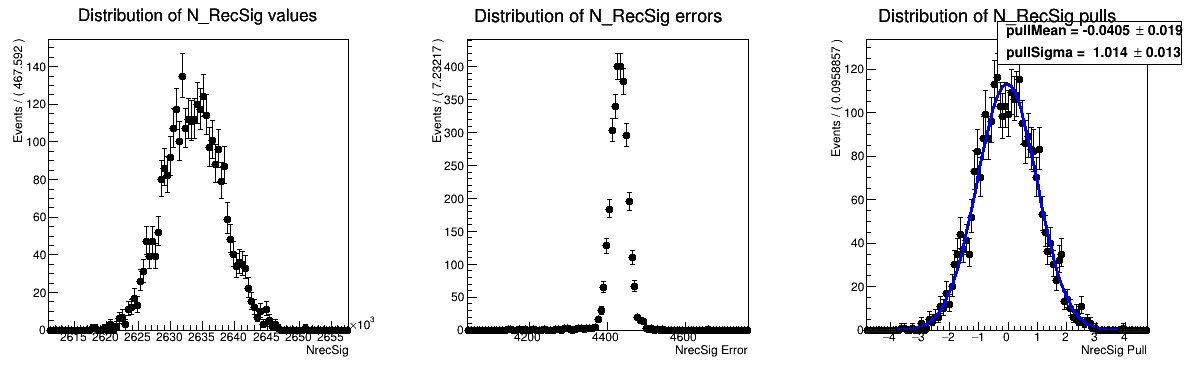
\includegraphics[width=14cm]{A3-Appendix/figs/NrecSigchargedBtag_mcstudy.png}
   % \caption{Fit on $M(p K \pi)$ in the region $5.25 < M_{bc} < 5.258$ GeV/c$^2$.  }
   % \label{fig:CrossfeedMbcRegionsInvMpeak1}
  \end{subfigure}
  \begin{subfigure}{15cm}
    \centering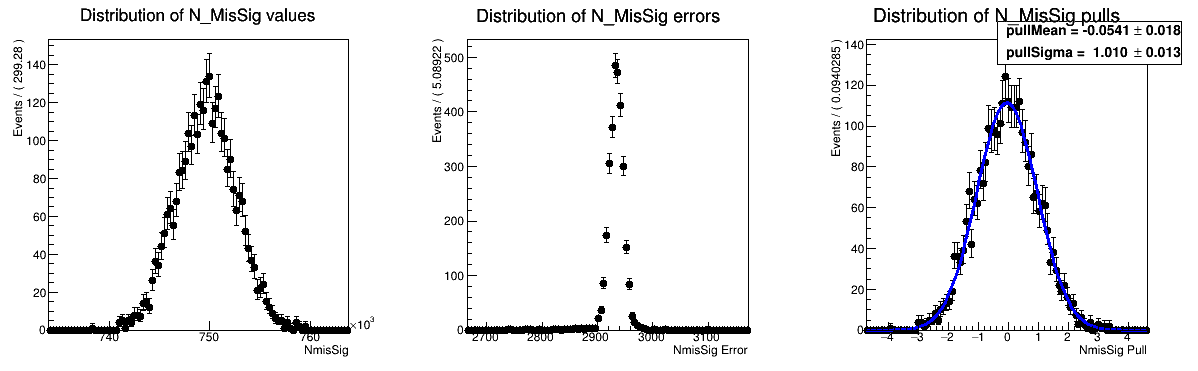
\includegraphics[width=14cm]{A3-Appendix/figs/NmisSigchargedBtag_mcstudy.png}
  \end{subfigure}

  \begin{subfigure}{15cm}
    \centering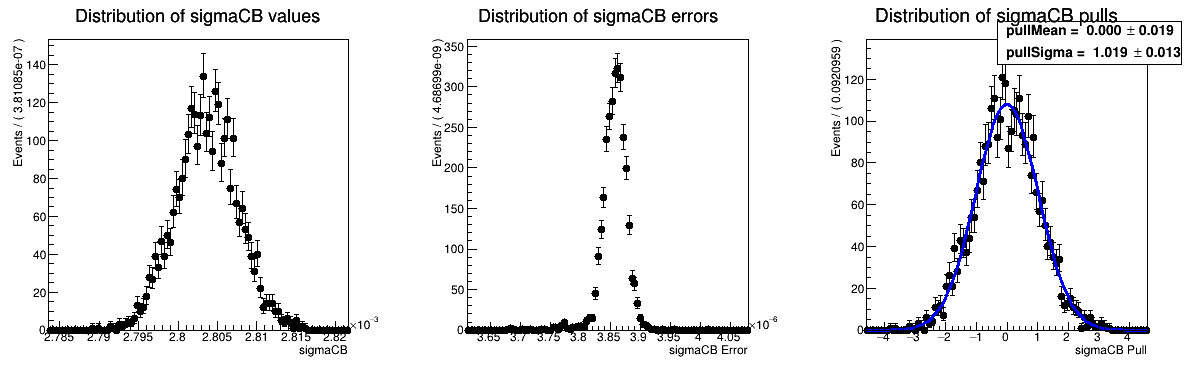
\includegraphics[width=14cm]{A3-Appendix/figs/sigmaCBchargedBtag_mcstudy.png}
  \end{subfigure}
  \begin{subfigure}{15cm}
    \centering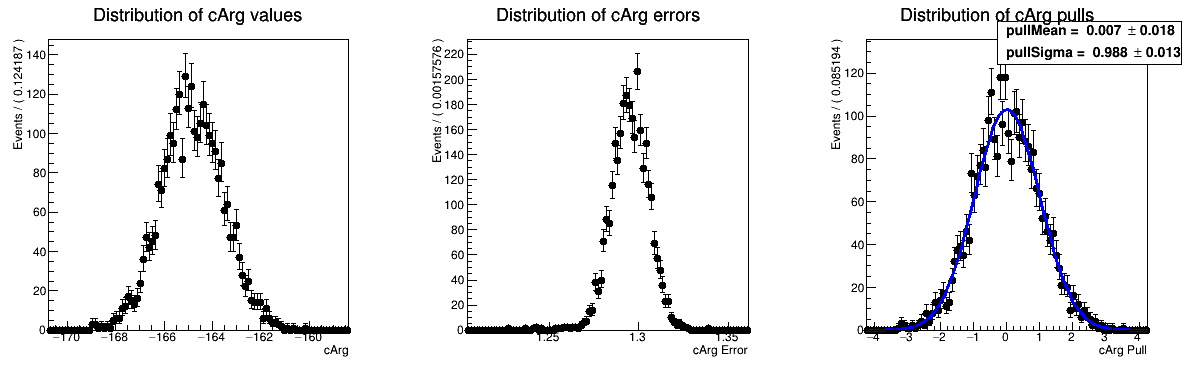
\includegraphics[width=14cm]{A3-Appendix/figs/cArg_chargedBtag_mcstudy.png}
    %\label{fig:CrossfeedMbcRegionsInvMpeak5}
  \end{subfigure}
  %\label{fig:CrossfeedMbcRegionsInvMpeak}
  \caption{Toy MC study for the $B_{tag}$ fit model described in Sec. \ref{sec:chargedAnticorrBtagFit}}
\end{figure}

